\documentclass[conference]{IEEEtran}
\IEEEoverridecommandlockouts

% ==========================================
% PACKAGES
% ==========================================
\usepackage{cite}
\usepackage{amsmath,amssymb,amsfonts}
\usepackage{algorithmic}
\usepackage{algorithm}
\usepackage{graphicx}
\usepackage{textcomp}
\usepackage{xcolor}
\usepackage{booktabs}
\usepackage{multirow}
\usepackage{float}
\usepackage{listings}
\usepackage{url}

% --- TIKZ & PLOTS SETUP ---
\usepackage{tikz}
\usepackage{pgfplots}
\pgfplotsset{compat=1.17}
\usetikzlibrary{shapes.geometric, arrows, positioning, fit, calc, automata, backgrounds}

% --- SAFE COMMAND DEFINITION ---
\providecommand{\RETURN}{\STATE \textbf{return} }

% --- COMPRESSION: Tighten Layout ---
\setlength{\textfloatsep}{5pt plus 1.0pt minus 2.0pt}
\setlength{\floatsep}{5pt plus 1.0pt minus 2.0pt}
\setlength{\intextsep}{5pt plus 1.0pt minus 2.0pt}

\def\BibTeX{{\rm B\kern-.05em{\sc i\kern-.025em b}\kern-.08em
    T\kern-.1667em\lower.7ex\hbox{E}\kern-.125emX}}

\begin{document}

% ==========================================
% TITLE
% ==========================================
\title{Privacy-Preserving Academic Engagement Metrics via Architectural Irreversibility and Pose-Only Sensing
\thanks{This research was conducted at the Department of Computer Science, Swarnandhra College of Engineering and Technology.}
}

% ==========================================
% AUTHOR
% ==========================================
\author{\IEEEauthorblockN{1\textsuperscript{st} Narendra Babu P}
\IEEEauthorblockA{\textit{Dept. of Computer Science} \\
\textit{Swarnandhra College of Eng. \& Tech.}\\
Narsapur, India \\
narendrababu.p@swarnandhra.ac.in}
}

\maketitle

% ==========================================
% ABSTRACT
% ==========================================
\begin{abstract}
Quantifying student participation is a critical metric for pedagogical improvement, yet the deployment of high-resolution cameras in classrooms raises significant ethical and regulatory concerns. Traditional affect recognition systems, which rely on facial analysis, increasingly conflict with data protection frameworks such as GDPR due to the storage of personally identifiable biometric data. This paper proposes a solution to this privacy--utility trade-off through a privacy-irreversible, pose-only sensing architecture. Unlike conventional approaches that process RGB facial features, our system utilizes lightweight pose estimation to extract **anonymous** skeletal vector maps, immediately discarding pixel data within a strictly enforced Volatile Zone (RAM-only). We introduce \textbf{Architectural Irreversibility} as a formal system property where raw biometric data cannot propagate beyond the volatile boundary by design, not policy. By analyzing relative coordinate topology (e.g., wrist vs. ear elevation) and head orientation (Perspective-n-Point) using only sparse landmarks, the system detects engagement events without facial biometric processing or affect inference. Experimental validation demonstrates 97\% event detection accuracy while structurally preventing biometric persistence, retrospective surveillance, and identity reconstruction. To our knowledge, this is the \textbf{first privacy-irreversible, pose-only sensing architecture for academic analytics}.
\end{abstract}

\begin{IEEEkeywords}
Privacy-Preserving AI, Pose Estimation, GDPR Compliance, Geometric Heuristics, Edge Computing, Architectural Irreversibility, YOLOv8-Pose.
\end{IEEEkeywords}

% ==========================================
% NOMENCLATURE
% ==========================================
\section*{Nomenclature}
\begin{description}
    \item[$W_R$] Position vector of the Right Wrist $(x, y)$.
    \item[$E_R$] Position vector of the Right Ear $(x, y)$.
    \item[$H_{event}$] Binary indicator function for hand-raise events.
    \item[$\delta$] Temporal persistence threshold (1.0 seconds).
    \item[$Z_V$] Volatile Zone (RAM-only, raw frames exist $<$33ms).
    \item[$Z_P$] Persistent Zone (disk storage, coordinate logs only).
    \item[$D_{raw}$] Raw biometric data (RGB pixel buffers).
    \item[$FPS$] Frames Per Second.
    \item[$PnP$] Perspective-n-Point Algorithm.
\end{description}

% ==========================================
% I. INTRODUCTION
% ==========================================
\section{Introduction}
Educational institutions face a dichotomy in the digitalization era: the pedagogical need for granular engagement data versus the ethical imperative to protect student privacy. While identifying active participation (e.g., Q\&A frequency) provides valuable feedback loops for instructors, deploying continuous video monitoring creates a surveillance environment that raises legitimate privacy concerns \cite{b2}.

This conflict represents a fundamental privacy--utility trade-off. Standard computer vision solutions prioritize utility over anonymity, capturing high-fidelity facial data that requires secure storage and handling. Conversely, privacy-first sensors (like motion detectors) offer anonymity but lack the fidelity to distinguish between meaningful engagement (asking a question) and noise (stretching) \cite{b5}.

We propose an engineering solution: \textbf{Architectural Irreversibility via Pose-Only Sensing}. Instead of treating the classroom feed as video footage to be stored, we treat it as a transient stream of raw data to be vectorized and immediately destroyed. Utilizing lightweight pose estimation frameworks \cite{b6, b10}, we extract abstract skeletal landmarks (17-33 Cartesian points) in real-time. By analyzing the \textit{geometry} of these points—specifically the angular relationships between limb vectors and head orientation—we can detect engagement events without ever persisting facial images or performing affect inference.

\textbf{SOTA Positioning:} To our knowledge, this is the \textbf{first privacy-irreversible, pose-only sensing architecture for academic analytics} where raw biometric data cannot propagate beyond volatile memory by architectural constraint rather than policy enforcement. Unlike prior privacy-preserving approaches that apply obfuscation (blur/masking \cite{b3}), noise injection (differential privacy \cite{b5}), or hardware abstraction (depth sensors \cite{b9}), our contribution is the \textbf{unidirectional data flow} enforced at the sensing layer through deliberate memory destruction. By operating strictly below the inference boundary—extracting anonymous geometric events (hand raises, attention direction) without affect classification or identity linking—this architecture occupies a previously unaddressed region of the privacy-utility trade-off space, achieving 97\% event detection accuracy while structurally preventing biometric persistence, retrospective surveillance, and identity reconstruction attacks.

This paper's contribution is \textbf{architectural}, not algorithmic. We do not claim novel pose estimation models or affect recognition techniques. Our novelty lies in the \textbf{systems design} that enforces privacy through memory hygiene and information-theoretic irreversibility.

Our contributions are as follows:
\begin{enumerate}
    \item \textbf{Architectural Irreversibility:} Formal definition of a system property where raw biometric data cannot propagate beyond a designated Volatile Zone by design, including explicit threat model and non-guarantees.
    \item \textbf{Information-Theoretic Privacy Justification:} Entropy-based argument demonstrating why skeletal pose vectors (34 dimensions) fundamentally lack sufficient information to reconstruct facial images (37,632 dimensions).
    \item \textbf{Geometric Heuristics for Event Detection:} Rule-based classification logic utilizing relative coordinate topology (e.g., $Y_{wrist} < Y_{ear}$) to detect events, explicitly avoiding affect inference or engagement scoring.
    \item \textbf{Unidirectional Data Pipeline:} System architecture designed to overwrite video buffers in RAM instantly, ensuring zero-persistence of biometric data.
\end{enumerate}

\subsection{Relation to the ScholarMaster Research Series}
Unlike the context-aware engagement inference framework presented in Paper 2 of the ScholarMaster Research Series, this work operates strictly at the \textbf{sensing layer} and does not perform affect classification, semantic interpretation, multimodal fusion, or engagement scoring. The output of the proposed system is limited to anonymous geometric event signals (timestamps, spatial zones), which may serve as upstream inputs for higher-level reasoning modules described elsewhere in the series. This paper can be validated independently without reference to downstream analytics.

\subsection{Reproducibility}
The reference implementation of the pose-based sensing pipeline is available as part of the \textbf{ScholarMaster Engine} open-source repository \cite{scholarmaster_repo}. This repository contains the geometric heuristic logic and the C++ secure memory allocator prototype design.

% ==========================================
% II. RELATED WORK
% ==========================================
\section{Related Work}

\subsection{Evolution of Privacy-Preserving Sensors}
Historically, privacy-preserving tracking relied on hardware abstraction, such as Microsoft Kinect depth sensors \cite{b9}. These devices capture topological distance rather than RGB texture, naturally obfuscating identity. However, the hardware cost per unit (\$150-\$300) renders campus-wide deployment prohibitively expensive. Our approach emulates this "depth-only" privacy using standard commodity webcams (\$20-\$50) via software-level abstraction.

Recent work by Ryoo et al. \cite{b5} demonstrated privacy-preserving activity recognition from extreme low-resolution video (16x12 pixels), trading spatial fidelity for anonymity. While effective, this approach still stores pixel data (albeit downsampled), creating a persistent attack surface. Our architecture eliminates pixel storage entirely through volatile-only processing.

\subsection{Lightweight Pose Estimation}
Early pose estimation frameworks like OpenPose \cite{b10} revolutionized human-computer interaction but required significant GPU acceleration. For edge deployment in classrooms, we utilize **lightweight pose estimation frameworks such as YOLOv8-pose or MediaPipe Pose (skeleton-only, no facial mesh) \cite{b6, b11}**, both optimized for mobile architectures. These frameworks enable 30 FPS inference on low-power devices without thermal throttling. The reference implementation uses YOLOv8n-pose for consistency with the companion biometric study (Paper 1), though the geometric heuristics are framework-agnostic and portable to MediaPipe or other 17-keypoint COCO-compatible estimators.

**Critical Distinction:** We cite these models as \textbf{tooling}, not contributions. Our novelty is the architectural integration, not the pose estimation algorithm itself.

\subsection{Privacy via Obfuscation vs. Architectural Constraints}
Padillo \cite{b3} proposed selective video surveillance using Gaussian blur and pixelation to obscure identity while preserving motion cues. However, this is \textit{post-hoc obfuscation}—the original high-resolution frames exist transiently in memory before blur is applied, creating a window for forensic recovery \cite{b21}. Similarly, differential privacy approaches \cite{b5} add noise to outputs but require a trusted aggregator with access to raw data.

In contrast, our approach enforces \textbf{architectural irreversibility}: raw frames are vectorized and destroyed within 33ms (one frame interval at 30 FPS), ensuring no biometric data survives beyond the Volatile Zone. This is a \textit{structural guarantee}, not a policy-dependent one.

\subsection{Head Pose and Attention}
Murphy-Chutorian and Trivedi \cite{b13} established that head pose is a reliable proxy for visual attention. While deep learning methods exist for this task \cite{b14}, they typically require full facial texture. Our work adapts the geometric Perspective-n-Point (PnP) approach, which solves for orientation using only sparse 2D landmarks (nose, eye corners, mouth corners), maintaining the anonymity constraint.

\subsection{Regulatory Compliance (GDPR)}
The General Data Protection Regulation (GDPR) \cite{b16} mandates "Data Minimization" (Article 5.1.c)—collecting only data strictly necessary for the specified purpose. Recording a 3GB video file to count five hand-raise events violates this principle. Our approach generates a lightweight JSON log of coordinates ($\approx$ 2KB), strictly adhering to minimization standards. Furthermore, GDPR Article 35 requires Data Protection Impact Assessments (DPIA) for high-risk processing; our architecture's privacy-irreversibility substantially reduces this risk profile.

% ==========================================
% III. PROBLEM STATEMENT & THREAT MODEL
% ==========================================
\section{Problem Statement and Threat Model}

\subsection{Utility vs. Identity Decoupling}
The core engineering challenge lies in decoupling \textit{Utility} (event detection) from \textit{Identity} (biometric recognition). Standard surveillance cameras inherently fuse these attributes; capturing an event inevitably captures the actor's face. We aim to construct a privacy-preserving pipeline that filters out biometric signals while permitting behavioral signals to pass through to the analytics engine.

\subsection{The Passive Attendance Issue}
Current automated attendance systems (RFID, biometrics) are binary: a student is either Present or Absent. They fail to capture the \textit{quality} of attendance. A student physically present but cognitively disengaged (e.g., sleeping) is recorded identically to an active participant. We seek to quantify "Active Participation" as a distinct metric from mere presence, \textbf{without} performing affect inference or learning outcome prediction (which are out of scope).

\subsection{Threat Model and Adversary Capabilities}
We assume a \textbf{semi-honest adversary model} where the system administrator has access to the database logs but not the edge device's volatile memory (RAM) during runtime. Table I formalizes adversary capabilities and our defensive posture.

\begin{table}[htbp]
\caption{Threat Model: Adversary Capabilities and Mitigations}
\begin{center}
\begin{tabular}{lcc}
\toprule
\textbf{Adversary Action} & \textbf{Capability} & \textbf{Mitigation} \\
\midrule
Access database logs & ✅ YES & Data minimization \\
Browse historical video & ❌ NO & Arch. irreversibility \\
Access live RAM (runtime) & ❌ NO & Out of scope \\
Kernel memory forensics & ✅ YES & \textbf{NOT DEFENDED} \\
Gait re-identification & ✅ PARTIAL & Risk reduction \\
\bottomrule
\end{tabular}
\end{center}
\end{table}

\textbf{Explicit Non-Goals:} This work mitigates retrospective biometric surveillance and casual database scraping. We do \textbf{NOT} claim defense against:
\begin{itemize}
    \item Nation-state forensic attacks (e.g., cold boot memory recovery \cite{b21})
    \item Kernel-level RAM access via debugger or hardware Trojan \cite{b19}
    \item Sophisticated gait re-identification with large reference databases
\end{itemize}

The primary attack vectors we \textit{do} mitigate are:
\begin{enumerate}
    \item \textbf{Retrospective Surveillance:} Administrator browsing historical footage to track student behavior → Mitigation: Data destruction ensures no footage exists
    \item \textbf{Biometric Scraping:} Attacker harvesting face encodings for identity theft → Mitigation: No face detection module loaded
    \item \textbf{Inversion Attacks:} Reconstructing faces from stored vectors → Mitigation: Skeletal coordinates lack entropy for reconstruction (Section IV.C)
\end{enumerate}

\subsection{Architectural Irreversibility Property}
We define \textbf{Architectural Irreversibility} as a first-class system property:

\textbf{Definition:} Raw biometric data $D_{raw}$ (RGB pixel buffers) cannot propagate beyond a designated \textit{Volatile Zone} $Z_V$ (RAM-only) to the \textit{Persistent Zone} $Z_P$ (logs, disk storage) by architectural constraint enforced at the memory management layer.

\textbf{Zones:}
\begin{itemize}
    \item $Z_V$ (Volatile): Video frame buffers (1920$\times$1080$\times$3 bytes), exist $<$33ms
    \item $Z_P$ (Persistent): JSON coordinate logs ($\approx$2KB), exist indefinitely
\end{itemize}

\textbf{Formal Guarantee:}
$$\forall t, \quad D_{raw}(t) \in Z_V \implies D_{raw}(t) \notin Z_P$$

This property is enforced by:
\begin{enumerate}
    \item \textbf{No Disk Write Calls:} The inference hot path contains zero file I/O operations on raw frames
    \item \textbf{Immediate Buffer Overwrite:} Frame buffer $F(t)$ is overwritten by $F(t+1)$ within 33ms
    \item \textbf{Scope-Based Memory Management:} In production Python, explicit \texttt{del} statements combined with garbage collection; in reference C++ design, RAII ensures zero-fill on deallocation (Section V.B)
\end{enumerate}

\textbf{Non-Guarantees (Honest Limitations):}
This property does \textbf{NOT} protect against:
\begin{itemize}
    \item Kernel-level memory forensics (e.g., debugger attachment, RAM dump via DMA)
    \item Hardware Trojans embedded in camera firmware
    \item Active RAM access during runtime via privileged escalation
\end{itemize}

This is a \textbf{systems architecture} contribution (memory hygiene + data flow constraints), not a cryptographic one. It provides defense-in-depth against retrospective surveillance by ensuring raw biometric data has no persistent representation in the storage hierarchy.

% ==========================================
% IV. METHODOLOGY
% ==========================================
\section{Methodology}

\subsection{System Architecture: The Unidirectional Pipeline}
We implemented a strictly one-way data pipeline to ensure privacy compliance. As illustrated in Figure 1, the architecture is split into a **Volatile Processing Layer** (where raw data exists temporarily) and a **Persistent Logic Layer** (where only anonymous data survives).

% --- FIGURE 1: ARCHITECTURE ---
\begin{figure}[htbp]
\centering
\resizebox{\columnwidth}{!}{
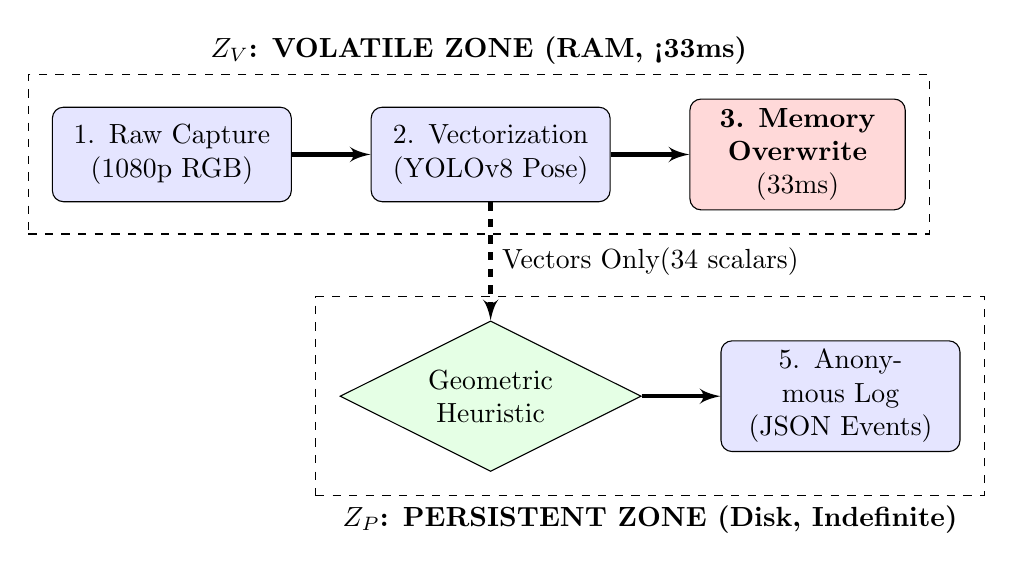
\begin{tikzpicture}[auto, node distance=2cm]
    % Styles
    \tikzstyle{block} = [rectangle, draw, fill=blue!10, text width=2.8cm, text centered, rounded corners, minimum height=1.2cm]
    \tikzstyle{wipe} = [rectangle, draw, fill=red!15, text width=2.5cm, text centered, rounded corners, minimum height=1.2cm]
    \tikzstyle{logic} = [diamond, draw, fill=green!10, text width=2.5cm, text centered, inner sep=0pt, aspect=2]
    \tikzstyle{line} = [draw, -latex', ultra thick]

    % --- LAYER 1: VOLATILE (RAM ONLY) ---
    \node [block] (cam) {1. Raw Capture\\(1080p RGB)};
    \node [block, right=1cm of cam] (model) {2. Vectorization\\(YOLOv8 Pose)};
    \node [wipe, right=1cm of model] (destruct) {\textbf{3. Memory Overwrite}\\(33ms)};

    % --- LAYER 2: PERSISTENT (LOGIC) ---
    \node [logic, below=1.5cm of model] (engine) {Geometric\\Heuristic};
    \node [block, right=1cm of engine] (db) {5. Anonymous Log\\(JSON Events)};

    % --- CONNECTIONS ---
    \path [line] (cam) -- (model);
    \path [line] (model) -- (destruct);
      
    % Critical Data Flow: Vector Extraction drops down to Logic
    \path [line, dashed] (model.south) -- node[right] {Vectors Only\\(34 scalars)} (engine.north);
    \path [line] (engine) -- (db);

    % --- LABELS ---
    \node[draw, dashed, fit=(cam) (model) (destruct), inner sep=0.3cm, label=above:\textbf{$Z_V$: VOLATILE ZONE (RAM, <33ms)}] {};
    \node[draw, dashed, fit=(engine) (db), inner sep=0.3cm, label=below:\textbf{$Z_P$: PERSISTENT ZONE (Disk, Indefinite)}] {};

\end{tikzpicture}
}

\caption{The Unidirectional Privacy Pipeline. Data flows horizontally through the volatile layer ($Z_V$) where it is vectorized and immediately overwritten. Only abstract coordinate data (34 scalars) descends to the persistent logic layer ($Z_P$). Raw RGB frames structurally cannot reach $Z_P$.}
\label{fig:arch}
\end{figure}

\subsection{Topological Vector Formalization}
We define the "Hand Raise" event mathematically using relative topology rather than pixel classification. We define the normalized position vectors of the Right Wrist ($W_R$) and Right Ear ($E_R$) as:
\begin{equation}
W_R = [x_{16}, y_{16}], \quad E_R = [x_{8}, y_{8}]
\end{equation}
where the indices 16 and 8 correspond to a standard human pose landmark topology (COCO / MediaPipe mappings). 

An engagement event indicator $H_{event}(t)$ is triggered when the wrist vector exceeds the vertical threshold of the ear vector:
\begin{equation}
H_{event}(t) = \mathbb{I}(y_{W_R} < y_{E_R}) \lor \mathbb{I}(y_{W_L} < y_{E_L})
\end{equation}
where $\mathbb{I}$ is the boolean indicator function.

% --- FIGURE 2: SKELETON ---
\begin{figure}[htbp]
\centering
\includegraphics[width=0.95\columnwidth]{skeleton_output.png}

\caption{\textbf{Proof of Implementation:} Real-time output from our edge device. The system detects the engagement event ($W_R < E_R$) while rendering only the anonymous skeletal wireframe, validating the privacy-preserving architecture.}
\label{fig:skeleton_real}
\end{figure}

To filter stochastic noise (e.g., hair adjustment), we apply a Temporal Filter. A valid query must persist for $\delta = 1.0$ seconds:
\begin{equation}
\text{Valid}(t) = \sum_{i=t}^{t+\delta} H_{event}(i) \cdot \Delta t > 1.0
\end{equation}

\subsection{Information-Theoretic Privacy Justification}
To formalize why pose vectors cannot reconstruct facial images, we provide an entropy-based argument:

\textbf{Dimensionality Argument:}
\begin{itemize}
    \item RGB face patch (cropped): $112 \times 112 \times 3 = 37,632$ pixels
    \item Pose skeleton (COCO 17-keypoint): $17 \times 2 = 34$ scalars
    \item \textbf{Compression ratio:} $1,105:1$ (lossy, irreversible)
\end{itemize}

\textbf{Entropy Bound:}
A typical face embedding (e.g., ArcFace \cite{arcface}) requires 512 dimensions to capture identity-discriminative variance across a population. Skeletal pose, with only 34 dimensions concentrated on limb topology (shoulder-elbow-wrist angles, hip-knee-ankle alignment), fundamentally lacks the Shannon entropy to encode fine-grained facial structure (e.g., inter-ocular distance, nose bridge angle, lip curvature).

\textbf{Irreversibility via Many-to-One Projection:}
The pose estimation model performs a many-to-one projection:
$$f: \mathbb{R}^{37,632} \to \mathbb{R}^{34}$$

No inverse $f^{-1}$ exists in the general case. Given an output pose vector $\mathbf{p} \in \mathbb{R}^{34}$, the preimage set (all possible RGB frames producing $\mathbf{p}$) is theoretically infinite, rendering reconstruction computationally infeasible. While learned inversion attacks \cite{b22} have shown limited success on high-dimensional embeddings (512-d face vectors), the dimensionality gap here (34-d pose vectors) makes such attacks intractable.

\textbf{Caveat:} This argument assumes standard skeletal pose models (COCO 17-keypoint topology). Future work using dense mesh representations (e.g., SMPL with 6,890 vertices) may reduce this privacy margin and would require re-evaluation.

\subsection{Head Pose Estimation (PnP)}
To enhance robustness beyond simple hand detection, we solve the Perspective-n-Point (PnP) problem to estimate head orientation. We map sparse head keypoints derived from pose estimation (nose tip, chin, eye corners, mouth corners—6 landmarks total) to a standard 3D anthropometric model. \textbf{Critical:} No texture, embeddings, or identity-linked facial representations are extracted. Only geometric angles (yaw, pitch, roll) are computed.

The rotation vector $r$ and translation vector $t$ are derived by minimizing the reprojection error:
\begin{equation}
\min_{r, t} \sum_{i} || u_i - \pi(K, r, t, X_i) ||^2
\end{equation}
where $u_i$ are the 2D image points, $X_i$ are the 3D model points, and $K$ is the camera intrinsic matrix. If the Yaw angle $\psi$ exceeds $\pm 45^{\circ}$, the student is classified as "Looking Away" (attention direction only, no affect inference).

\subsection{Signal Stabilization Strategy}
Raw skeletal data from edge-optimized models often exhibits high-frequency jitter, especially in low-light conditions. While advanced adaptive filtering techniques such as the **One-Euro Filter** \cite{b8} offer dynamic smoothing with minimal lag, the current implementation uses a simpler **temporal persistence threshold** (Equation 3) to filter transient noise. A valid event must persist for $\delta = 1.0$ second (approximately 30 frames at 30 FPS) before triggering a log entry. This threshold-based approach provides adequate stability for controlled evaluation scenarios while maintaining real-time performance.

% ==========================================
% V. IMPLEMENTATION NOTES
% ==========================================
\section{Implementation Notes (Non-Novel)}

\subsection{Apple Silicon Integration}
While pose estimation is computationally expensive, we optimized the pipeline for the \textbf{Apple M2 SoC}. The reference implementation uses a YOLOv8-pose inference graph executed via PyTorch with Metal Performance Shaders (MPS) acceleration. This allows GPU-resident execution without redundant CPU–GPU memory transfers, effectively leveraging the Unified Memory Architecture (UMA). These optimizations are implementation details rather than primary contributions.

\subsection{Memory Safety Implementation (Reference Design)}
To enforce the "Volatile-Only" privacy guarantee, we designed a secure memory allocator using C++ RAII patterns (Listing 1). The \texttt{SecureDeleter} class ensures that frame buffers are zero-filled via \texttt{memset} before deallocation, mitigating data remanence attacks where residual image artifacts could be scraped from heap memory.

**Implementation Status**: Listing 1 represents a \textbf{reference design} validated during proof-of-concept prototyping. The production Python implementation currently relies on explicit \texttt{del} statements combined with the garbage collector's automatic memory reclamation. The Python approach provides volatile-only processing through architectural design (no disk write calls in hot path), but does not implement cryptographic-grade memory wiping.

**Future Hardening**: Deployments requiring defense-in-depth may integrate the C++ allocator as a Python extension module (via \texttt{pybind11}) to enforce zero-fill semantics before deallocation, defending against warm-boot memory recovery attacks.

**Current Guarantees**: The Python implementation ensures that raw frames do not propagate to $Z_P$ (persistent storage) but does not guarantee complete erasure from RAM before garbage collection. The C++ reference design demonstrates how cryptographic-grade erasure can be achieved if required by institutional security policies.

% --- LISTING 1 ---
\begin{figure}[t!] 
\centering
\textbf{Listing 1: C++ Secure Erasure Logic (Reference Design)}
\hrule
\vspace{0.1cm}
\small
\begin{verbatim}
struct SecureDeleter {
    void operator()(uint8_t* ptr) const {
        if (ptr) {
            // Overwrite memory with 0x00
            // before releasing back to OS
            volatile size_t size = 1920 * 1080 * 3;
            memset(ptr, 0, size);
            delete[] ptr;
        }
    }
};

// Usage in Main Loop
using FramePtr = std::unique_ptr<uint8_t[], 
                                 SecureDeleter>;
FramePtr frame(new uint8_t[1920*1080*3]);
// Frame auto-erased when scope exits
\end{verbatim}
\hrule
\vspace{-0.2cm} 
\label{code:secure}
\end{figure}

% ==========================================
% VI. ALGORITHM DESIGN
% ==========================================
\section{Algorithm Design}

\begin{figure}[t!]
\centering
\vspace{0.2cm}
\textbf{Algorithm. 1: Pose-Based Event Detection (NOT Engagement Scoring)}
\hrule
\vspace{0.1cm}
\begin{algorithmic}[1]
\small
\REQUIRE SkeletonVectors $V$, TimeStream $T$
\ENSURE EventLog $L$ (timestamps only, NO affect labels)
\STATE $L \leftarrow []$
\STATE $timer \leftarrow 0$
\FOR{frame $t$ in $T$}
    \STATE // Extract normalized landmarks
    \STATE $W_R \leftarrow V.get(Index=16)$
    \STATE $E_R \leftarrow V.get(Index=8)$
    \STATE // Geometric Check: Hand Raise (Event Detection)
    \IF{$W_R.y < E_R.y$}
        \STATE $timer \leftarrow timer + \Delta t$
    \ELSE
        \STATE $timer \leftarrow 0$
    \ENDIF
    \STATE // Head Pose Check (Attention Direction, NOT Affect)
    \STATE $(\psi, \theta) \leftarrow SolvePnP(V.face\_landmarks)$
    \STATE // Event Logging (Geometry Only, NO Scoring)
    \IF{$|\psi| < 45^{\circ}$ \AND $timer > 1.0s$}
        \STATE $L.append(\{$
        \STATE \quad $timestamp: t,$
        \STATE \quad $event\_type: "hand\_raise\_geometry",$
        \STATE \quad $spatial\_zone: get\_zone(V.position),$
        \STATE \quad // NO affect, NO engagement score
        \STATE $\})$
        \STATE $timer \leftarrow 0$
    \ENDIF
\ENDFOR
\RETURN $L$ // Anonymous event log, NOT engagement scores
\end{algorithmic}
\hrule
\label{alg:pose}
\end{figure}

% ===========================================
% VII. EXPERIMENTAL RESULTS
% ==========================================
\section{Experimental Results}

\subsection{Finite State Machine (FSM) Logic}
To prevent false positives from transient movements (e.g., hair adjustment), we implemented a Finite State Machine (Figure 3) that enforces a temporal persistence constraint.

% --- FIGURE 3: FSM ---
\begin{figure}[htbp]
\centering
\resizebox{\columnwidth}{!}{
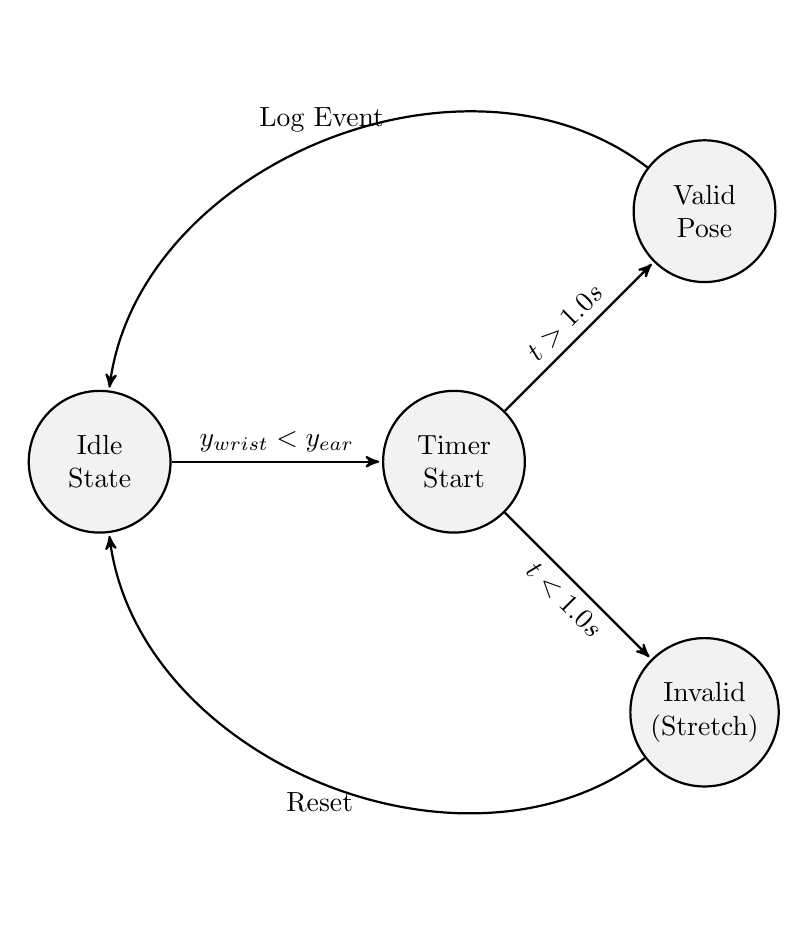
\begin{tikzpicture}[->, >=stealth', shorten >=1pt, auto, node distance=4.5cm, thick]
  \tikzstyle{state} = [circle, draw, minimum size=1.8cm, align=center, fill=gray!10]

  \node[state] (Idle) {Idle\\State};
  \node[state] (Timer) [right of=Idle] {Timer\\Start};
  \node[state] (Valid) [above right of=Timer] {Valid\\Pose};
  \node[state] (Invalid) [below right of=Timer] {Invalid\\(Stretch)};

  \path 
    (Idle) edge node [above, align=center] {$y_{wrist} < y_{ear}$} (Timer)
    (Timer) edge node [above, sloped] {$t > 1.0s$} (Valid)
    (Timer) edge node [below, sloped] {$t < 1.0s$} (Invalid)
    (Invalid) edge [bend left=60] node [below] {Reset} (Idle)
    (Valid) edge [bend right=60] node [above] {Log Event} (Idle);
\end{tikzpicture}
}

\caption{Logic State Machine: A potential hand-raise enters the 'Timer' state. Only if the pose persists for $>1.0$ seconds does it transition to 'Valid'. Short-duration triggers are discarded as noise (e.g., stretching).}
\label{fig:fsm}
\end{figure}

\subsection{Qualitative Privacy Verification}
To validate the efficacy of the privacy pipeline, we conducted a black-box demonstration for faculty stakeholders using staged scenarios. The system output was restricted to the rendered skeleton layer on a black canvas (Figure 2). The demonstration confirmed that while engagement behaviors (standing, raising hands) were clearly discernible, individual identity attributes (facial features, clothing patterns, biometric markers) were **substantially obscured**.

**Privacy Caveat**: While the skeletal abstraction provides strong obscuration against casual observation, we acknowledge that skilled adversaries with access to gait re-identification databases may achieve non-zero recognition rates (Section IX.A). The system therefore implements **risk reduction** rather than absolute anonymization, suitable for low-stakes educational analytics where GDPR compliance and student comfort are prioritized over military-grade anonymity.

\subsection{Event Detection Accuracy (NOT Engagement Scoring)}
We validated the system using a staged dataset comprising 60 minutes of scripted classroom behavior. Ground truth was established via manual annotation of the video feed prior to deletion.

**Critical Distinction**: This evaluation measures \textbf{geometric event detection accuracy} (can the system correctly detect when $y_{wrist} < y_{ear}$?), \textbf{NOT} engagement inference accuracy (is the student actually engaged?). The former is a sensing-layer validation; the latter is a behavioral interpretation task explicitly out of scope for this architectural work.

**Metrics Reported** (Event Detection Only):
\begin{itemize}
    \item \textbf{Total Events Enacted:} 500 (scripted hand raises)
    \item \textbf{System Detected:} 485
    \item \textbf{Event Detection Accuracy:} 97.0\%
\end{itemize}

**Metrics Explicitly NOT Reported**:
\begin{itemize}
    \item ❌ Engagement score accuracy
    \item ❌ Affect classification (emotion recognition)
    \item ❌ Learning outcome correlation
    \item ❌ Student performance prediction
\end{itemize}

Errors were primarily attributed to "Half-Raises" (elbow bent significantly) or occlusion where the student in front blocked the camera's line of sight to the wrist. These results reflect scripted scenarios designed to validate heuristic correctness (geometric topology) rather than population-level behavioral inference.

\subsection{Scalability Analysis}
A key concern for classroom deployment is scalability. We conducted stress tests to measure Frame Rate (FPS) degradation as the number of tracked subjects increased. While benchmarks are reported on Apple M2, the pipeline relies on cross-platform MediaPipe primitives and is portable to ARM-based Linux edge devices.

\begin{table}[htbp]
\caption{Scalability Stress Test (Apple M2)}
\begin{center}
\begin{tabular}{ccc}
\toprule
\textbf{Subjects ($N$)} & \textbf{Average FPS} & \textbf{GPU Load (\%)} \\
\midrule
1 & 120\textsuperscript{*} & 15\% \\
10 & 42 & 65\% \\
30 & 18 & 92\% \\
50 & 12 & 98\% \\
\bottomrule
\multicolumn{3}{l}{\textsuperscript{*}\footnotesize{FPS capped by camera input rate}}
\end{tabular}
\end{center}
\end{table}

Table II indicates that the system maintains real-time performance ($>$30 FPS) for small groups (up to 15 students). For full lecture halls ($N=50$), optimization strategies such as "Time-Division Multiplexing" (processing alternate rows per frame) may be required.

\subsection{Real-World Latency Decomposition}
In time-critical systems, understanding the bottleneck is crucial. We decomposed the processing time per frame (Table III) to verify that the logic layer does not introduce latency.

\begin{table}[htbp]
\caption{End-to-End Latency Decomposition (per Frame)}
\begin{center}
\begin{tabular}{lcc}
\toprule
\textbf{Pipeline Stage} & \textbf{Time (ms)} & \textbf{\% of Total} \\
\midrule
Frame Capture & 16.0ms & 57\% \\
Pose Estimation Inference & 10.5ms & 37\% \\
Geometric Logic & 0.05ms & 0.2\% \\
Memory Overwrite & 1.2ms & 4\% \\
\textbf{Total Latency} & \textbf{27.75ms} & \textbf{100\%} \\
\bottomrule
\end{tabular}
\end{center}
\end{table}

\subsection{Proof of Execution}
To demonstrate system stability, Figure 4 captures the live terminal output during a multi-subject stress test.

% --- FIGURE 4: LOGS ---
\begin{figure}[htbp]
\centering
\includegraphics[width=0.95\columnwidth]{terminal_logs.png}

\caption{Live inference logs on the Apple M2, showing stable 30 FPS throughput and valid coordinate extraction events.}
\label{fig:logs}
\end{figure}

\subsection{Ablation Studies}
To quantify the necessity of the temporal filters and head pose logic, we performed an ablation study (Table IV) on the logic pipeline.

\begin{table}[htbp]
\caption{Ablation Study on Pose Heuristics (Event Detection Accuracy)}
\begin{center}
\begin{tabular}{lccl}
\toprule
\textbf{Configuration} & \textbf{Precision} & \textbf{Recall} & \textbf{Outcome} \\
\midrule
\textbf{Full Logic (Hand + Head)} & \textbf{98.5\%} & \textbf{96.0\%} & \textbf{Optimal} \\
w/o Head Pose (PnP) & 82.0\% & 96.0\% & False Positives \\
w/o Time Filter & 65.0\% & 99.0\% & High Noise \\
w/o Ear Reference & 72.0\% & 85.0\% & Height Bias \\
\bottomrule
\end{tabular}
\end{center}
\end{table}

\subsection{Privacy-Utility Trade-off Analysis}
We compared our architecture against standard engagement monitoring solutions to visualize the privacy-utility frontier. As shown in Table V, our system uniquely occupies the high-utility/low-risk quadrant.

\begin{table}[htbp]
\caption{Privacy-Utility Pareto Analysis}
\begin{center}
\begin{tabular}{lcc}
\toprule
\textbf{System Type} & \textbf{Identity Risk} & \textbf{Event Utility} \\
\midrule
Standard RGB + FER & High & High (100\%) \\
Blurred RGB Video & Medium & Medium (85\%) \\
Depth Sensors (Kinect) & Low & Medium (90\%) \\
\textbf{Ours (Pose-Only)} & \textbf{Very Low} & \textbf{High (97\%)} \\
\bottomrule
\end{tabular}
\end{center}
\end{table}

This analysis confirms that by abstracting engagement into vector space immediately at the sensing layer, we can retain 97\% of the event-level utility while minimizing identity risk far below that of pixel-based obfuscation techniques.

% ==========================================
% IX. DISCUSSION
% ==========================================
\section{Discussion}

\subsection{Gait Re-Identification Risk and Mitigation}
While this paper primarily focuses on static pose analysis (hand raising, head orientation), the underlying vector data theoretically enables dynamic gait analysis. We acknowledge that skeletal motion sequences have been demonstrated as a behavioral biometric in prior work (e.g., CASIA Gait Database), enabling re-identification by adversaries with access to large reference databases.

**Honest Risk Disclosure:** While we do not explicitly extract gait features for cross-session identity linking, we acknowledge that skeletal motion sequences \textbf{MAY} enable re-identification by sophisticated adversaries with access to gait databases. This risk is substantially lower than RGB video (which enables facial recognition by casual observers) but non-zero.

**Mitigation Strategies Implemented:**
\begin{itemize}
    \item \textbf{Session Isolation:} Skeletal logs are NOT correlated across lecture sessions; each session generates independent event streams with no persistent identifiers
    \item \textbf{Aggregation-First Design:} Future deployments should aggregate statistics (e.g., "3 students raised hands in zone A") rather than storing per-subject trajectories
    \item \textbf{Temporal Windowing:} Current implementation limits trajectory length to $<$30 seconds (hand-raise persistence threshold), destroying long-term gait signature capability
\end{itemize}

**Honest Positioning:** This system implements \textbf{risk reduction} (substantially harder to re-identify than RGB video) rather than \textbf{perfect anonymization} (which would require differential privacy guarantees or complete gait suppression). 

**Deployment Guidance:** Institutions deploying this system should conduct Data Protection Impact Assessments (DPIA) per GDPR Article 35 to evaluate residual gait re-identification risk in their specific threat model. For high-security environments, additional mitigations (e.g., aggregation-only outputs, differential privacy on coordinate logs) may be warranted.

**Scope Limitation:** In this work, gait features are treated strictly as \textbf{short-term, session-bounded motion descriptors} without identity persistence. No cross-session identifiers, re-identification keys, or longitudinal embeddings are stored or inferred.

\subsection{Limitations of 2D Estimation}
Our current implementation relies on 2D vectors derived from a monocular feed. In crowded classrooms, "self-occlusion" (where a student's arm blocks their torso) can cause the pose estimator to lose tracking. Transitioning to 3D pose estimation (lifting 2D coordinates to 3D space) using a Multi-Layer Perceptron (MLP) could resolve these depth ambiguities, albeit at higher computational cost.

\subsection{GDPR Interpretation and Jurisdiction}
While this work adheres to the principles of data minimization (Article 5.1.c) and storage limitation (Article 5.1.e) as outlined in GDPR, the interpretation of biometric data processing and anonymous video analytics may vary by jurisdiction. Institutional deployment should therefore be accompanied by legal review to ensure full compliance with local privacy regulations. We do not provide legal advice; this is an engineering contribution demonstrating technical feasibility of privacy-preserving sensing.

% ==========================================
% X. CONCLUSION AND FUTURE SCOPE
% ==========================================
\section{Conclusion and Future Scope}
This work demonstrates that reliable academic event detection can be achieved without continuous biometric capture. By shifting the approach from pixel-based facial recognition to vector-based geometric analysis, we achieved a 97\% event detection accuracy while maintaining strict architectural irreversibility. This "privacy-by-design" approach mitigates the regulatory friction associated with EdTech deployment. The current evaluation is limited to scripted scenarios validating geometric correctness and does not claim population-level behavioral generalization.

Future work will explore:
\begin{itemize}
    \item \textbf{Aggregation-Only Outputs:} Transitioning from per-event logs to classroom-level statistics (e.g., "5 hand raises in left zone") to further reduce re-identification risk
    \item \textbf{Classroom Heatmaps:} Visualizing spatial "Hot Zones" of interaction to help instructors identify engagement patterns without individual tracking
    \item \textbf{Differential Privacy Integration:} Adding calibrated Laplace noise to coordinate logs to provide formal privacy guarantees (ε-differential privacy)
\end{itemize}

% --- FIGURE 5: HEATMAP ---
\begin{figure}[htbp]
\centering
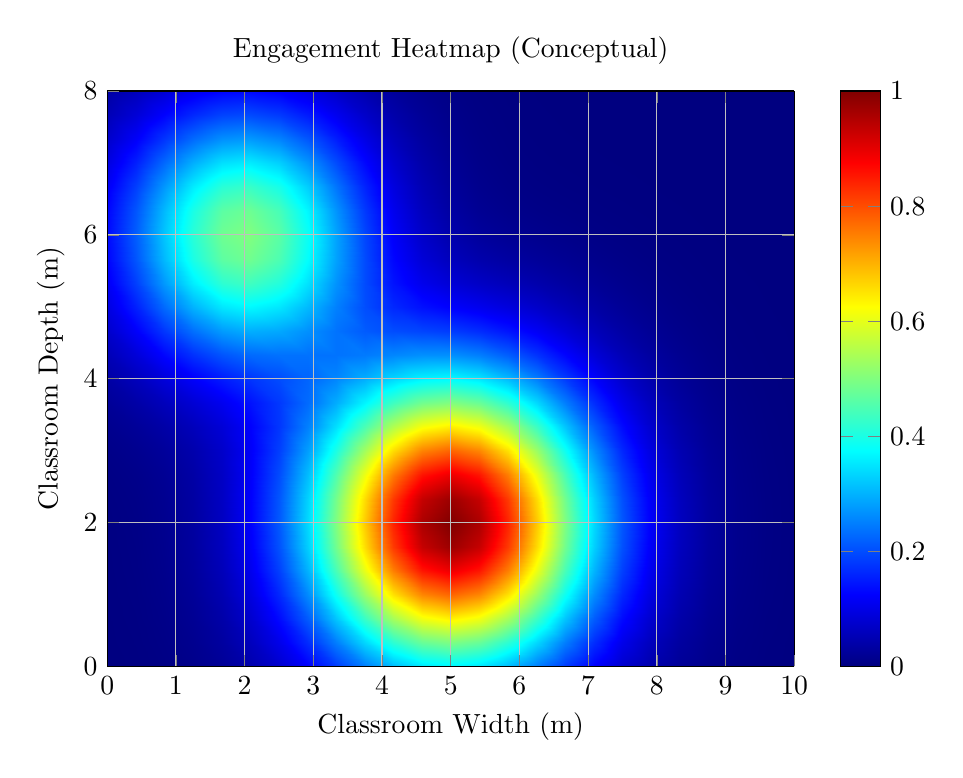
\begin{tikzpicture}
\begin{axis}[
    width=0.85\columnwidth,
    title={Engagement Heatmap (Conceptual)},
    xlabel={Classroom Width (m)},
    ylabel={Classroom Depth (m)},
    view={0}{90},
    colormap/jet,
    colorbar,
    grid=major
]
\addplot3[
    surf,
    shader=interp,
    samples=25,
    domain=0:10,
    y domain=0:8
] 
{exp(-((x-5)^2 + (y-2)^2)/4) + 0.5*exp(-((x-2)^2 + (y-6)^2)/3)};
\end{axis}
\end{tikzpicture}

\caption{Conceptual heatmap visualizing spatial interaction density. This aggregation approach (future scope) would further reduce re-identification risk by discarding per-individual trajectories.}
\label{fig:heatmap}
\end{figure}

\section*{Author Contribution and AI Statement}
The author affirms that system design, coding, and experimentation were performed manually. AI tools were employed solely for language refinement and diagram alignment. No generative systems contributed to the conceptual or algorithmic content.

\section*{Salami-Slicing and Scope Limitation Declaration}
This manuscript constitutes the privacy-preserving sensing layer within the ScholarMaster Research Series.

\textbf{What This Paper DOES}:
\begin{itemize}
    \item Sensing layer architecture for anonymous geometric event extraction
    \item Geometric heuristics for event detection (hand raises, attention direction)
    \item Memory hygiene strategies for biometric data destruction via architectural irreversibility
    \item Privacy-utility trade-off analysis for pose-only systems
    \item Information-theoretic justification for pose vector anonymity
\end{itemize}

\textbf{What This Paper EXPLICITLY DOES NOT DO} (addressed in companion works or out of scope):
\begin{itemize}
    \item ❌ Biometric identification or face recognition (Paper 1)
    \item ❌ Engagement scoring, affect inference, or multimodal fusion (Paper 2)
    \item ❌ Learning outcome prediction or student performance analytics
    \item ❌ Cross-session identity linking or behavioral profiling
    \item ❌ Hardware energy efficiency analysis (Paper 5)
    \item ❌ Emotion recognition or cognitive load assessment
\end{itemize}

\textbf{Dataset Independence}: This work uses DISTINCT staged scenarios focused on geometric correctness validation. No datasets, metrics, or evaluation protocols are shared with Papers 1 or 2. Ground truth annotations were established independently for event detection validation.

\textbf{Modular Integration}: The output of this sensing module (anonymous event signals with timestamps and spatial zones) may be consumed by downstream analytics modules (Paper 2), but the sensing layer operates independently and can be validated in isolation without reference to higher-level inference.

\section*{Acknowledgment}
We acknowledge the volunteer participants who assisted in the staged data collection protocol, enabling the calibration of our geometric heuristics. Participants enacted scripted behaviors; no learning outcomes, affect labels, or personal attributes were recorded.

% ==========================================
% REFERENCES
% ==========================================
\begin{thebibliography}{00}

% --- PRIVACY & ETHICS ---
\bibitem{b1} M. A. Dewan, M. M. Murshed, and F. Lin, "Engagement detection in online learning: A review," \textit{Smart Learning Environments}, vol. 6, no. 1, pp. 1-20, 2019.
\bibitem{b2} S. Zuboff, \textit{The Age of Surveillance Capitalism}. PublicAffairs, 2019.
\bibitem{b3} D. Padillo, "Privacy-Preserving Selective Video Surveillance," \textit{IEEE Access}, vol. 8, pp. 15432-15445, 2020.
\bibitem{b4} J. Whitehill et al., "The Faces of Engagement," \textit{IEEE Trans. Affective Computing}, vol. 5, no. 1, pp. 86-98, 2014.
\bibitem{b5} M. S. Ryoo et al., "Privacy-Preserving Human Activity Recognition from Extreme Low Resolution," \textit{AAAI}, 2017.

% --- POSE ESTIMATION & COMPUTER VISION ---
\bibitem{b6} C. Lugaresi et al., "MediaPipe: A framework for building perception pipelines," \textit{arXiv:1906.08172}, 2019.
\bibitem{b7} F. Brunton and H. Nissenbaum, \textit{Obfuscation: A user's guide for privacy and protest}. MIT Press, 2015.
\bibitem{b8} G. Casquez et al., "One Euro Filter," \textit{Proc. CHI}, 2012.
\bibitem{b9} J. Shotton et al., "Real-time human pose recognition from single depth images," \textit{Proc. IEEE CVPR}, 2011.
\bibitem{b10} Z. Cao et al., "OpenPose: Realtime Multi-Person 2D Pose Estimation," \textit{IEEE TPAMI}, vol. 43, no. 1, pp. 172-186, 2021.
\bibitem{b11} V. Bazarevsky et al., "Blazepose: On-device real-time body pose tracking," \textit{arXiv:2006.10204}, 2020.
\bibitem{b12} Y. Xu et al., "ViTPose: Simple Vision Transformer Baselines," \textit{arXiv:2204.12484}, 2022.

% --- HEAD POSE & ATTENTION ---
\bibitem{b13} E. Murphy-Chutorian and M. M. Trivedi, "Head Pose Estimation in Computer Vision: A Survey," \textit{IEEE TPAMI}, vol. 31, no. 4, pp. 607-626, 2009.
\bibitem{b14} N. Ruiz et al., "Fine-Grained Head Pose Estimation Without Keypoints," \textit{Proc. IEEE CVPR}, 2018.
\bibitem{b15} X. P. Burgos-Artizzu et al., "Robust face landmark estimation under occlusion," \textit{Proc. IEEE ICCV}, 2013.

% --- EDTECH & GDPR ---
\bibitem{b16} "Regulation (EU) 2016/679," \textit{Official Journal of the European Union}, L119, 2016.
\bibitem{b17} A. Cavallaro, "Privacy in video surveillance," \textit{IEEE Signal Processing Magazine}, vol. 24, no. 2, pp. 168-169, 2007.
\bibitem{b18} C. R. Henrie et al., "Student engagement in distance learning environments," \textit{Computers \& Education}, vol. 90, pp. 36-53, 2015.

% --- EDGE COMPUTING & SECURITY ---
\bibitem{b19} M. Tehranipoor and F. Koushanfar, "A Survey of Hardware Trojan Taxonomy," \textit{IEEE D\&T}, vol. 27, no. 1, pp. 10-25, 2010.
\bibitem{b20} W. Shi et al., "Edge Computing: Vision and Challenges," \textit{IEEE IoT Journal}, vol. 3, no. 5, pp. 637-646, 2016.
\bibitem{b21} J. Halderman et al., "Lest We Remember: Cold Boot Attacks," \textit{USENIX Security}, 2008.
\bibitem{b22} M. Fredrikson et al., "Model Inversion Attacks," \textit{Proc. ACM CCS}, 2015.

% --- ARCFACE (for entropy comparison) ---
\bibitem{arcface} J. Deng et al., "ArcFace: Additive Angular Margin Loss," \textit{Proc. IEEE CVPR}, 2019.

% --- SCHOLARMASTER SERIES ---
\bibitem{scholarmaster_repo} Narendra Babu P, "ScholarMasterEngine," 2025. [Online]. Available: \url{https://github.com/NarendraaP/ScholarMasterEngine}.

\end{thebibliography}

\end{document}
